\documentclass[../main.tex]{subfiles}
\begin{document}
\chapter{Basics Of Vectors}
\section{Definition and Axioms}
\subsection{Introductory Definitions}
A vector is specified by a (positive) magnitude and a direction in space.
We can represent a vector as line segment between two points $A$ and $B$, $\vec{v} = \avec{AB}$.
$\vec{v}$ has length $|\vec{v}|$ and direction from $A$ to $B$.
If we chose an origin $O$ then considering a point $A$ it has position vector denoted $\vec{a} = \avec{OA}$.
\label{vectorSpaceDef}
\begin{definition}[Vector Space]
  A \textit{vector space}, $V$, over $\R$ or $\C$ is a collection of vectors $\vec{v} \in V$, together with two operations:
  \begin{enumerate}
    \item Addition of two vectors
    \item Multiplication by a scalar (from $\R$ or $\C$ respectively)
  \end{enumerate}
\end{definition}
Vector addition has to satisfy the following axioms:
\begin{enumerate}
  \item \textbf{Commutativity -} $\vec{a} + \vec{b} = \vec{b} + \vec{a}$
  \item \textbf{Associativity -} $(\vec{a} + \vec{b}) + \vec{c} = \vec{a} + (\vec{b} + \vec{c})$
  \item \textbf{Identity -} There exists a vector $\vec{0}$ such that for all $a \in V$, $\vec{a} + \vec{0} = \vec{a}$
  \item \textbf{Inverse -} For all vectors $\vec{a} \in V$, there is a vector ($-\vec{a}$) such that $\vec{a} + (-\vec{a}) = \vec{0}$.
\end{enumerate}
Scalar multiplication has to satisfy the following axioms (Where $\lambda$ and $\mu$ are scalars):
\begin{enumerate}
  \item $\lambda(\vec{a} + \vec{b}) = \lambda \vec{a} + \lambda \vec{b}$
  \item $(\lambda + \mu)\vec{a} = \lambda \vec{a} + \mu \vec{a}$
  \item $\lambda(\mu \vec{a}) = (\lambda \mu)\vec{a}$
  \item $1(\vec{a}) = \vec{a}$
\end{enumerate}
\begin{remark}
  Vectors under addition are an abelian group.
\end{remark}
\begin{remark}[Warning]
  $\R^{n}$ is a vector space with addition (component-wise) and scalar multiplication.
  We can represent $\R$ by a line and this could make us think that any line is a vector space however this is not true as the space does not necessarily contain $O$.
  E.g. $x + y = d$ is not a vector space.
\end{remark}

\subsection{Geometric View}
Given vectors $\vec{a}$ and $\vec{b}$ which are the position vectors of $A$ and $B$ respectively, we can construct the parallelogram $OACB$:
\begin{center}
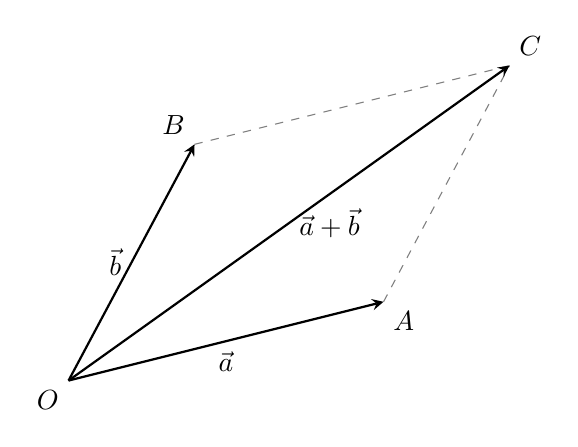
\begin{tikzpicture}[scale=2,>=stealth]
  \coordinate (O) at (0,0);
  \coordinate (A) at (2,0.5);   % vector a
  \coordinate (B) at (0.8,1.5); % vector b
  \coordinate (C) at (2.8,2);   % a + b

  \node[below left] at (O) {$O$};
  \node[below right] at (A) {$A$};
  \node[above left] at (B) {$B$};
  \node[above right] at (C) {$C$};

  \draw[->, thick, black] (O) -- (A) node[midway, below] {$\vec{a}$};
  \draw[->, thick, black] (O) -- (B) node[midway, left] {$\vec{b}$};

  \draw[dashed, gray] (A) -- (C);
  \draw[dashed, gray] (B) -- (C);

  \draw[->, thick, black] (O) -- (C) node[midway, right] {$\vec{a} + \vec{b}$};
\end{tikzpicture}
\end{center}

and then $\vec{a} + \vec{b} = \vec{c}$, where $\vec{c}$ is the position vector of $C$.

Given a vector $\vec{a}$ which is the position vector of a point $A$ and a $\lambda \in \R$.
$\lambda \vec{a}$ is a position vector of a point on the line through $OA$, with length $|\lambda \vec{a}| = |\lambda||\vec{a}$.

\begin{center}
\begin{tikzpicture}[scale=2,>=stealth]
  \coordinate (O) at (0,0);
  \coordinate (A) at (1.2,0.6);
  \coordinate (B) at (2.4,1.2);
  \coordinate (C) at (-1.2,-0.6);

  % Guide line
  \draw[dashed, gray] (-1.6,-0.8) -- (3,1.5);

  % Original vector
  \draw[->, thick, black] (O) -- (A) node[midway, below right] {$\vec{a}$};

  % Scaled vector
  \draw[->, black] (O) -- (B) node[near end, below right] {$\lambda \vec{a}$};

  % Reversed vector
  \draw[->, black] (O) -- (C) node[near end, below right] {$-\frac{\lambda}{2} \vec{a}$};

  % Label points
  \fill (O) circle (0.03);
  \node[below right] at (O) {$O$};
  \node[below right] at (A) {$A$};
\end{tikzpicture}
\end{center}
\begin{remark}[Note]
  $\{\lambda \vec{a}: \lambda \in \R\}$ is the set of all points on the line through $OA$.
\end{remark}

\subsection{Linear Combination and Span}
\begin{definition}[Linear Combination]
  Given $n$ vectors $\vec{r}_1, \vec{r}_2, \ldots, \vec{r}_n$, a \textit{linear combination} of those vectors is a vector of the form:
  \[
    \sum_{i = 1}^{n} \lambda_i \vec{r}_i  = \lambda_1 \vec{r}_1 + \lambda_2 \vec{r}_2 + \cdots + \lambda_n \vec{r}_n
  \]
  where $\lambda_1, \lambda_2, \ldots, \lambda_n$ are scalars.
\end{definition}
We can also define the ``space'' of all linear combinations of a set of vectors:
\begin{definition}[Span]
  Given $n$ vectors $\vec{r}_1, \vec{r}_2, \ldots, \vec{r}_n$, their \textit{span} is the set of all linear combinations of those vectors.
  \[
    \Span\{\vec{r}_1, \vec{r}_2, \ldots, \vec{r}_n\} = \left\{\sum_{i = 1}^{n} \lambda_i \vec{r}_i : \lambda_i \in K\right\}
  \]
  where $K$ is either $\C$ or $\R$ depending on the vector space.
\end{definition}
\begin{definition}[Parallel]
  Any two vectors $\vec{a}$ and $\vec{b}$ are \textit{parallel} if $\vec{a} = \lambda \vec{b}$ or $\vec{b} = \lambda \vec{a}$ for some $\lambda \in \R$.
  We denote this $\vec{a} \parallel \vec{b}$.
\end{definition}
\begin{remark}[Note]
  Since we allow $\lambda = 0$, $\vec{0} \parallel \vec{a}$ for any $\vec{a}$.
\end{remark}
If $\vec{a} \centernot\parallel \vec{b}$ ($\vec{a}$ and $\vec{b}$ are not parallel), then $\Span\{\vec{a}, \vec{b}\}$ is a plane through $O$, $A$, and $B$.
\begin{definition}[Unit Vector]
  A \textit{unit vector} is a vector with length $1$.
  They are denoted $\uvec{v}$.
\end{definition}
\section{Scalar Product}
The \textit{scalar product} of two vectors within a vector space returns a scalar (either real or complex).
\subsection{Geometric Viewpoint in \texorpdfstring{$\R^{n}$}{Real Vector Spaces}}
First consider the usual scalar product in $\R^{n}$.
\begin{definition}[Scalar Product]
  The \textit{scalar product} of two vectors $\vec{a}$ and $\vec{b}$ is defined as:
  \[
    \vec{a} \cdot \vec{b} = |\vec{a}||\vec{b}|\cos\theta
  \]
  where $\theta$ is the angle between $\vec{a}$ and $\vec{b}$.
\end{definition}
\begin{remark}[Note]
  If $|\vec{a}| = 0$ or $|\vec{b}| = 0$ then $\theta$ is not well defined, but in that case we have $\vec{a} \cdot \vec{b} = 0$.
\end{remark}
Intuitively the dot product is the product of the parts of $\vec{a}$ and $\vec{b}$ that are parallel.

The scalar product in $\R^{n}$ satisfies the following properties:
\begin{enumerate}
  \item $\vec{a} \cdot \vec{b} = \vec{b} \cdot \vec{a}$
  \item $\vec{a} \cdot \vec{a} = |\vec{a}|^2 \geq 0$ (and $|\vec{a}| = 0 \iff \vec{a} = \vec{0}$)
  \item $(\lambda \vec{a}) \cdot \vec{b} = \lambda (\vec{a} \cdot \vec{b}) = \vec{a} \cdot (\lambda \vec{b})$
  \item $\vec{a} \cdot (\vec{b} + \vec{c}) = \vec{a} \cdot \vec{b} + \vec{a} \cdot \vec{c}$
\end{enumerate}
\begin{definition}[Orthogonal]
  Any two vectors $\vec{a}$ and $\vec{b}$ are \textit{orthogonal} or \textit{perpendicular} if $\vec{a} \cdot \vec{b} = 0$.
  We denote this $\vec{a} \perp \vec{b}$.
\end{definition}
\begin{remark}[Note]
  We also also allow $\vec{a} = \vec{0}$ or $\vec{b} = \vec{0}$ and hence $\vec{0}$ is orthogonal to any other vector.
\end{remark}
\begin{definition}[Projection]
  Given two vectors $\vec{a}$ and $\vec{b}$, the projection of $\vec{b}$ onto $\vec{a}$ is:
  \[
    \uvec{a}|\vec{b}|\cos \theta = (\uvec{a} \cdot \vec{b}) \uvec{a}
  \]
\end{definition}

\begin{center}
\begin{tikzpicture}[scale=2,>=stealth]
  \coordinate (O) at (0,0);
  \coordinate (A) at (2,0);
  \coordinate (B) at (1.2,1.4);
  \coordinate (P) at (1.2,0);

  % vectors a and b
  \draw[->, black] (O) -- (A) node[near end, below] {$\vec{a}$};
  \draw[->, black] (O) -- (B) node[midway, left] {$\vec{b}$};

  % projection line
  \draw[dashed, gray] (B) -- (P);

  % projection of b onto a
  \draw[->, thick, black] (O) -- (P) node[midway, below] {$\underbrace{(|\vec{b}|\cos\theta)\uvec{a}}_{\text{projection of $\vec{b}$ onto $\vec{a}$}}$};

  % angles
  \draw (0.5,0) arc[start angle=0, end angle=49, radius=0.5];
  \node at (0.6,0.2) {$\theta$};
  \draw ($(P)+(0,0.1)$) -- ($(P)+(0.1,0.1)$) -- ($(P)+(0.1,0)$);
\end{tikzpicture}
\end{center}
We can use the scalar product to quickly derive the cosine rule:
\begin{proof}
  \begin{align*}
    |\avec{BC}|^2 &= |\avec{AC} - \avec{AB}|^2 \\
                  &= (\avec{AC} - \avec{AB}) \cdot (\avec{AC} - \avec{AB}) \\
                  &= |\avec{AC}|^2 - 2 \avec{AB} \cdot \avec{AC} + |\avec{AB}|^2 \\
                  &= |\avec{AC}|^2 + |\avec{AB}|^2 - 2 |\avec{AB}||\avec{AC}|\cos\theta
  \end{align*}
\end{proof}
\subsection{General Algebraic Viewpoint}
This definition generalises to any other vector space, keeping the same axioms.
\begin{definition}[Inner/Scalar Product]
  In a real vector space $V$, an \textit{inner product} or \textit{scalar product} is a map $V \times V \to \R$ that satisfies:
  \begin{enumerate}
    \item \textbf{Symmetry -} $\vec{x} \cdot \vec{y} = \vec{y} \cdot \vec{x}$
    \item \textbf{Linearity in 2nd Argument -} $\vec{x} \cdot(\lambda \vec{y} + \mu \vec{z}) = \lambda \vec{x} \cdot \vec{y} + \mu \vec{x} \cdot \vec{z}$
    \item \textbf{Positive Definiteness - } $\vec{x} \cdot \vec{x} \geq 0$ with equality if and only if $\vec{x} = \vec{0}$
  \end{enumerate}
  We denote it either $\vec{x} \cdot \vec{y}$ or $\inner{\vec{x}}{\vec{y}}$.
\end{definition}
\begin{remark}[Note]
  We get linearity in the first argument also because of symmetry.
\end{remark}
\begin{definition}[Norm]
  The norm of a vector $\vec{a}$ is given by $\sqrt{\vec{a} \cdot \vec{a}}$.
  We denote this as either $|\vec{a}|$ or $\norm{\vec{a}}$.
\end{definition}
\begin{theorem}[Cauchy-Schwarz Inequality]
  For all $\vec{x}, \vec{y} \in \R^{n}$,
  \[
    |\vec{x} \cdot \vec{y}| \leq |\vec{x}||\vec{y}|
  \]
\end{theorem}
\begin{proof}
  Consider the expression $|x - \lambda y|^2$, $\lambda \in \R$.
  Then,
  \begin{align*}
    |\vec{x} - \lambda\vec{y}|^2 &\geq 0 \\
    (\vec{x} - \lambda \vec{y}) \cdot (\vec{x} - \lambda \vec{y}) &\geq 0 \\
    \abs{\vec{x}}^2 + \lambda^2 \abs{\vec{y}}^2 - 2\lambda \vec{x} \cdot \vec{y} &\geq 0 \\
    (\lambda^2 \abs{\vec{y}}^2 - 2 \vec{x} \cdot \vec{y} \lambda + \abs{\vec{x}}^2) &\geq 0
  \end{align*}
  This quadratic always needs to be non-negative so we require the discriminant to be less than or equal to zero.
  \begin{align*}
    4(\vec{x} \cdot \vec{y})^2 - 4 \abs{\vec{x}}^2 \abs{\vec{y}}^2 &\leq 0 \\
    \abs{\vec{x} \cdot \vec{y}} &\leq \abs{\vec{x}} \abs{\vec{y}}
  \end{align*}
\end{proof}
Notice that this proof holds for all possible scalar products on any real vector space as we only used the axioms of the scalar product.
\begin{remark}
  Equality ($\abs{\vec{x} \cdot \vec{y}} = \abs{\vec{x}}\abs{\vec{y}}$) holds if and only if $\vec{x} = \lambda \vec{y}$ or $\vec{y} = \lambda \vec{x}$ for some $\lambda \in \R$ (i.e. $\vec{x}$ and $\vec{y}$ are parallel).
\end{remark}
We can now set:
\[
  \vec{x} \cdot \vec{y} = |\vec{x}||\vec{y}|\cos\theta
\]
to define the angle between $\vec{x}$ and $\vec{y}$ in $\R^{n}$ since Cauchy-Schwarz ensures that $-1 \leq \cos \theta \leq 1$.
\begin{corollary}[Triangle Inequality]
  For two vectors $\vec{x}, \vec{y}$
  \[
    \abs{\vec{x} + \vec{y}} \leq \abs{\vec{x}} + \abs{\vec{y}}
  \]
\end{corollary}
\begin{proof}
  \begin{align*}
    \abs{\vec{x} + \vec{y}}^2 &= (\vec{x} + \vec{y}) \cdot (\vec{x} + \vec{y}) \\
                              &= \abs{\vec{x}}^2 + \abs{\vec{y}}^2 + 2 \vec{x} \cdot \vec{y} \\
                              &\leq \abs{\vec{x}}^2 + \abs{\vec{y}}^2 + 2 \abs{\vec{x}}\abs{\vec{y}} \\
                              &= (\abs{\vec{x}} + \abs{\vec{y}})^2
  \end{align*}
  Therefore $\abs{\vec{x} + \vec{y}} \leq \abs{\vec{x}} + \abs{\vec{y}}$.
\end{proof}

\section{Orthonormal Bases}
\label{orthonormalBasis}
\begin{remark}[Note]
For this section, consider vectors in $\R^{3}$ only.
\end{remark}
Consider vectors $\vec{e}_1, \vec{e}_2, \vec{e}_3$ that are orthonormal:
\[
  \abs{\vec{e}_1} = \abs{\vec{e}_2} = \abs{\vec{e}_3} = 1 \text{ and } \vec{e}_i \cdot \vec{e}_j = \begin{cases}
  1 & i=j \\
  0 & i\neq j
  \end{cases}
\]
That is, they are all length 1 and are mutually orthogonal.
This is called an \textit{orthonormal basis} and is equivalent to choosing Cartesian axes along these directions.
There are infinitely many choices for an orthonormal basis in $\R^{3}$.

Any vector in $\R^{3}$ can be written as a combination of these:
\[
  \vec{a} = \sum_{i}^{} a_i \vec{e}_i = a_1 \vec{e}_1 + a_2 \vec{e}_2 + a_3 \vec{e}_3
\]
Each component of $\vec{a}$ is uniquely determined by $a_i = \vec{e}_i \cdot \vec{a}$

We will denote $\vec{a}$ as either a row vector or a column vector:
\[
  \vec{a} = (a_1, a_2, a_3) \text{ or } \vec{a} =
  \begin{pmatrix}
  a_1 \\
  a_2 \\
  a_3 \\
  \end{pmatrix}
\]
Now for $\vec{a}, \vec{b} \in \R^{3}$:
\begin{align*}
  \vec{a} \cdot \vec{b} &= (a_1 \vec{e}_1 + a_2 \vec{e}_2 + a_3 \vec{e}_3) \cdot (b_1 \vec{e}_1 + b_2 \vec{e}_2 + b_3 \vec{e}_3) \\
                        &= a_1 b_1 + a_2 b_2 + a_3 b_3
\end{align*}
In particular:
\[
  \vec{a} \cdot \vec{a} = \abs{\vec{a}}^2 = a^{2}_{1} + a^{2}_{2} + a^{2}_{3}
\]

The \textit{canonical basis} of $\R^{3}$, the one we use for the representation in terms of row or column vectors is:
\[
  \vec{e}_1 = (1, 0, 0),\; \vec{e}_2 = (0, 1, 0),\; \vec{e}_3 = (0, 0, 1)
\]
\begin{remark}[Notation]
The canonical orthonormal basis vectors for $\R^{3}$ are usually denoted $\uvec{i}$, $\uvec{j}$, $\uvec{k}$.
\end{remark}

\section{Vector Product}
\begin{remark}[Note]
For this section, consider vectors in $\R^{3}$ only.
\end{remark}
\subsection{Definition}
\begin{definition}[Vector Product]
  Consider $\vec{a}, \vec{b} \in \R^{3}$. The \textit{vector product} is defined by:
  \[
    \vec{a} \times \vec{b} = \abs{\vec{a}} \abs{\vec{b}}(\sin\theta)\uvec{n}
  \]
  Where $\uvec{n}$ is a unit vector that is orthogonal to both $\vec{a}$ and $\vec{b}$ and $\theta$ is the angle between $\vec{a}$ and $\vec{b}$.
  It is sometimes denoted $\vec{a} \wedge \vec{b}$.
\end{definition}
\begin{remark}[Right-Hand Rule]
  If $\vec{a}$ is on your first finger and $\vec{b}$ is on your second finger then $\vec{a} \times \vec{b}$ points in the direction of your thumb.
\end{remark}

\begin{center}
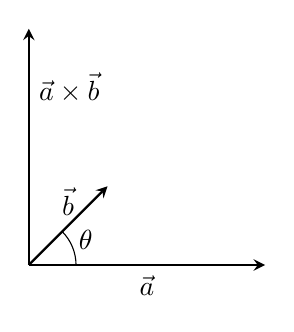
\begin{tikzpicture}[>=stealth]
\draw[thick,->] (0,0) -- (3,0) node[midway,below] {$\vec{a}$};
\draw[thick,->] (0,0) -- (1,1) node[midway,above] {$\vec{b}$};
\draw[thick,->] (0,0) -- (0,3) node[near end,right] {$\vec{a}\times \vec{b}$};
\draw (0.6,0) arc [start angle=0,end angle=45,radius=0.6] node[pos=0.7,right] {$\theta$};
\end{tikzpicture}
\end{center}
\begin{remark}
  $\uvec{n}$ is not defined if $\vec{a}$ and $\vec{b}$ are parallel but $\theta = 0 \text{ or } \pi$ so $\vec{a} \times \vec{b} = \vec{0}$.

  $\theta$ is not defined if $\abs{\vec{a}} = 0$ or $\abs{\vec{b}} = 0$ but then $\vec{a} \times \vec{b} = \vec{0}$ regardless.
\end{remark}
Some properties of the vector product are:
\begin{enumerate}
  \item $\vec{a} \times \vec{b} = - \vec{b} \times \vec{a}$ (Anti-symmetric)
  \item $\vec{a} \times \vec{a} = \vec{0}$
  \item $\vec{a} \times \vec{b} = 0 \iff \vec{a} = \lambda \vec{b}$ for some $\lambda \in \R$
  \item $(\lambda \vec{a}) \times \vec{b} = \lambda (\vec{a} \times \vec{b}) = \vec{a} \times (\lambda \vec{b})$
  \item $\vec{a} \times (\vec{b} + \vec{c}) = \vec{a} \times \vec{b} + \vec{a} \times \vec{c}$
  \item $\vec{a} \cdot (\vec{a} \times \vec{b}) = \vec{b} \cdot (\vec{a} \times \vec{b}) = 0$
\end{enumerate}
\subsection{Geometric Uses}
For vectors $\vec{a}, \vec{b}$ then $\vec{a} \times \vec{b}$ is the vector area of the parallelogram.
For example with $\sin \theta \geq 0$ we have:
\[
  \abs{\vec{a} \times \vec{b}} = \abs{\vec{a}} \abs{\vec{b}} \sin \theta = \text{base} \times \text{perpendicular height} = \text{area}
\]
\begin{center}
\begin{tikzpicture}[scale=3,>=stealth]
\coordinate (O) at (0,0);
\coordinate (A) at (2,0);
\coordinate (B) at (1.2,1.2);
\coordinate (H) at (1.2,0);

\fill[gray!20] (O) -- (A) -- ($(A)+(B)$) -- (B) -- cycle;

\draw[<->, dashed] (B) -- (H) node[midway,right] {$\abs{\vec{b}}\sin\theta$};

\draw (0.3,0) arc (0:45:0.3);
\node at (0.4,0.15) {$\theta$};

\node at (2.3,0.9) {$\abs{\vec{a} \times \vec{b}}$};
\draw[->, thick] (O) -- (A) node[midway, below] {$\vec{a}$};
\draw[->, thick] (O) -- (B) node[midway, above left] {$\vec{b}$};

\draw[dashed] (A) -- ($(A)+(B)$);
\draw[dashed] (B) -- ($(A)+(B)$);
\end{tikzpicture}
\end{center}
This can also be used to find the area of triangle $OAB = \frac{1}{2} \abs{\vec{a} \times \vec{b}}$.
\begin{center}
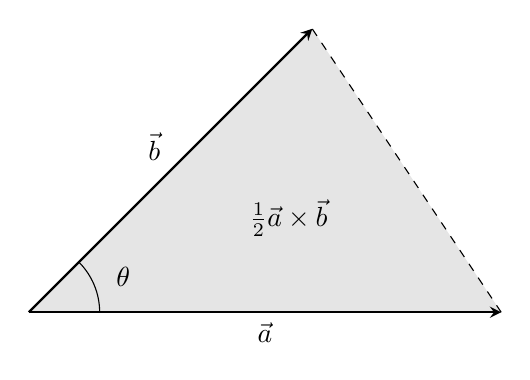
\begin{tikzpicture}[scale=3,>=stealth]
\coordinate (O) at (0,0);
\coordinate (A) at (2,0);
\coordinate (B) at (1.2,1.2);
\coordinate (H) at (1.2,0);

\fill[gray!20] (O) -- (A) -- (B) -- cycle;

\draw (0.3,0) arc (0:45:0.3);
\node at (0.4,0.15) {$\theta$};

\node at (1.1,0.4) {$\frac{1}{2}\abs{\vec{a} \times \vec{b}}$};
\draw[->, thick] (O) -- (A) node[midway, below] {$\vec{a}$};
\draw[->, thick] (O) -- (B) node[midway, above left] {$\vec{b}$};
\draw[dashed] (A) -- (B);
\end{tikzpicture}
\end{center}
We can also fix a vector $\vec{a}$ and consider $\vec{a} \perp \vec{x}$. Then computing $\vec{a} \times \vec{x}$ gives another vector that scales $\vec{x}$ by $|\vec{a}|$ and rotates it by $\pi/2$ in a plane that is orthogonal to $\vec{a}$.
\begin{center}
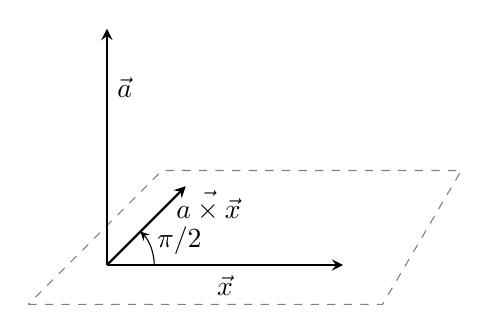
\begin{tikzpicture}[>=stealth]
\draw[gray, dashed] (-1,-0.5) -- (3.5, -0.5) -- (4.5, 1.2) -- (0.7, 1.2) -- cycle;
\draw[thick,->] (0,0) -- (3,0) node[midway,below] {$\vec{x}$};
\draw[thick,->] (0,0) -- (1,1) node[near end,right] {$\vec{a \times \vec{x}}$};
\draw[thick,->] (0,0) -- (0,3) node[near end,right] {$\vec{a}$};
\draw[->] (0.6,0) arc [start angle=0,end angle=45,radius=0.6] node[pos=0.7,right] {$\pi/2$};
\end{tikzpicture}
\end{center}

\subsection{Component Expressions}
Consider an orthonormal basis $\vec{e}_1, \vec{e}_2, \vec{e}_3$ from \cref{orthonormalBasis}.
If we impose the further restriction that:
\begin{align*}
  \vec{e}_1 \times \vec{e}_2 &= \vec{e}_3 = -\vec{e}_2 \times \vec{e}_1 \\
  \vec{e}_2 \times \vec{e}_3 &= \vec{e}_1 = -\vec{e}_3 \times \vec{e}_2 \\
  \vec{e}_3 \times \vec{e}_1 &= \vec{e}_2 = -\vec{e}_3 \times \vec{e}_1
\end{align*}
Then this is a \textit{right-handed} orthonormal basis.
Now consider $\vec{a} = (a_1, a_2, a_3)$ and $\vec{b} = (b_1, b_2, b_3)$ then:
\begin{align*}
  \vec{a} \times \vec{b} &= (a_1 \vec{e}_1 + a_2 \vec{e}_2 + a_3 \vec{e}_3) \times (b_1 \vec{e}_1 + b_2 \vec{e}_2 + b_3 \vec{e}_3) \\
                         &= (a_1 b_2 \vec{e}_3 - a_1 b_3 \vec{e}_2 - a_2 b_1 \vec{e}_3 + a_2 b_3 \vec{e}_1 + a_3 b_1 \vec{e}_2 - a_3 b_2 \vec{e}_1) \\
                         &= (a_2 b_3 - a_3 b_2) \vec{e}_1 + (a_3 b_1 - a_1 b_3) \vec{e}_2 + (a_1 b_2 - a_2 b_1) \vec{e}_3
\end{align*}
We can also write this as a matrix determinant:
\[
  \vec{a} \times \vec{b} =\begin{vmatrix}
  \vec{e}_1 & \vec{e}_2 & \vec{e}_3 \\
  a_1 & a_2 & a_3 \\
  b_1 & b_2 & b_3 \\
  \end{vmatrix}
\]
\section{Triple Products}
\begin{remark}[Note]
For this section, consider vectors in $\R^{3}$ only.
\end{remark}
\subsection{Scalar Triple Product}
\begin{definition}
  Consider $\vec{a}, \vec{b}, \vec{c}$ then the \textit{scalar triple product} is:
  \[
    [\vec{a}, \vec{b}, \vec{c}] = \vec{a} \cdot (\vec{b} \times \vec{c})
  \]
\end{definition}
Cyclic permutations of $\vec{a}, \vec{b}, \vec{c}$ retain the value of the scalar triple product and then swapping any two elements otherwise introduces a minus sign:
\begin{align*}
  &\vec{a} \cdot (\vec{b} \times \vec{c}) = \vec{b} \cdot (\vec{c} \times \vec{a}) = \vec{c} \cdot (\vec{a} \times \vec{b}) \\
  &= -\vec{a} \cdot (\vec{c} \times \vec{b}) = -\vec{b} \cdot (\vec{a} \times \vec{c}) = -\vec{c} \cdot (\vec{b} \times \vec{a})
\end{align*}
Geometrically, $|\vec{a} \cdot (\vec{b} \times \vec{c})|$ is the volume of the parallelepiped with sides $\vec{a}$, $\vec{b}$, $\vec{c}$.
\[
  |\vec{a} \cdot (\vec{b} \times \vec{c})| = (\text{area of base}) \times(\text{perpendicular height}) = \text{volume}
\]
If this is taken without the modulus then $\vec{a} \cdot (\vec{b} \times \vec{c})$ is a signed volume.
\begin{itemize}
  \item $\vec{a} \cdot (\vec{b} \times \vec{c}) > 0$ then $\vec{a}, \vec{b}, \vec{c}$ constitute a right handed set.
  \item $\vec{a} \cdot (\vec{b} \times \vec{c}) < 0$ then $\vec{a}, \vec{b}, \vec{c}$ constitute a left handed set.
  \item $\vec{a} \cdot (\vec{b} \times \vec{c}) = 0$ if and only if $\vec{a}, \vec{b}, \vec{c}$ are coplanar. That is, one of them is a linear combination of the other two.
\end{itemize}
\subsection{Vector Triple Product}
\begin{definition}[Vector Triple Product]
  $\vec{a}, \vec{b}, \vec{c} \in \R^{3}$ then the \textit{vector triple product} is:
  \[
    \vec{a} \times (\vec{b} \times \vec{c}) = (\vec{a} \cdot \vec{c}) \vec{b} - (\vec{a} \cdot \vec{b}) \vec{c}
  \]
\end{definition}
\begin{remark}[Warning]
  In general the vector triple product is not associative:
  \begin{align*}
    \vec{a} \times (\vec{b} \times \vec{c}) &= (\vec{a} \cdot \vec{c}) \vec{b} - (\vec{a} \cdot \vec{b})\vec{c} \\
    (\vec{a} \times \vec{b}) \times \vec{c} &= (\vec{a} \cdot \vec{c}) \vec{b} - (\vec{b} \cdot \vec{c})\vec{a}
  \end{align*}
\end{remark}
\section{Lines, Planes, and Vector Equations}
\subsection{Lines}
Any point on the line through a point $\vec{a}$ with direction $\vec{u}$ ($\vec{u} \neq 0$) has position vector given by:
\[
  \vec{r} = \vec{a} + \lambda \vec{u} \quad \lambda \in \R
\]

\begin{center}
\begin{tikzpicture}[scale=2,>=stealth]
  \coordinate (O) at (0.6,-0.5);
  \coordinate (A) at (0,0);
  \coordinate (B) at (2.4,1.2);
  \coordinate (C) at (1.2,0.6);

  \draw[dashed, gray] (-1.6,-0.8) -- (3,1.5);

  \draw[->, thick, black] (A) -- (C) node[midway, above left] {$\vec{u}$};
  \draw[->, thick, black] (O) -- (A) node[midway, above right] {$\vec{a}$};
  \draw[->, thick, black] (O) -- (B) node[midway, below right] {$\vec{r}$};
  \draw[->, black] (A) -- (B) node[near end, above left] {$\lambda \vec{u}$};


  \fill (O) circle (0.03);
  \node[below right] at (O) {$O$};
  \node[above left] at (A) {$A$};
\end{tikzpicture}
\end{center}
We can rearrange this to get:
\begin{align*}
  (\vec{r} - \vec{a}) &= \lambda \vec{u} \\
  (\vec{r} - \vec{a}) \times \vec{u} &= \vec{0}
\end{align*}
or equivalently $\vec{r} \times \vec{u} = \vec{b}$.
\subsection{Planes}
Any point on a plane though $\vec{a}$ with two direction vectors $\vec{u}$, $\vec{v}$ ($\vec{u} \centernot\parallel \vec{v}$) has position vector given by:
\[
  \vec{r} = \vec{a} + \lambda \vec{u} + \mu \vec{v} \quad \lambda, \mu \in \R
\]
A vector normal to the plane is given by $\vec{n} = \vec{u} \times \vec{v}$. Then we can write:
\[
  \vec{r} \cdot \vec{n} = \vec{a} \cdot \vec{n} \text{ or } (\vec{r} - \vec{a}) \cdot \vec{n} = 0
\]
The component of $\vec{r}$ along $\vec{n}$ is
\[
  \uvec{n} \cdot \vec{r} = \frac{\vec{n} \cdot \vec{r}}{|\vec{n}|} = \frac{k}{|\vec{n}|}
\]
The perpendicular distance from the origin to the plane is $\frac{|k|}{|n|}$.

If $\vec{a}, \vec{b}, \vec{c}$ are coplanar, then we can write the plane containing them as:
\[
  (\vec{r} - \vec{a}) \cdot [(\vec{b} - \vec{a}) \times (\vec{c} - \vec{a})] = 0
\]
\begin{example}[Finding the Intersection Between a Line and a Plane]
  Consider a line given by $\vec{u} \times \vec{r} = \vec{u} \times \vec{a}$ and a plane given by $\vec{n} \cdot \vec{r} = \vec{n} \cdot \vec{b}$.

  The line can also be written as $\vec{r} \times \vec{u} = \vec{a} \times \vec{u}$.
  Taking the vector product of this with $\vec{n}$ yields:
  \begin{align*}
    (\vec{a} \times \vec{u}) \times \vec{n} &= (\vec{r} \times \vec{u}) \times \vec{n}\\
                                            &= (\vec{r} \cdot \vec{n}) \vec{u} - (\vec{u} \cdot \vec{n}) \vec{r} \text{ by vector triple product}\\
                                            &= (\vec{b} \cdot \vec{n}) \vec{u} - (\vec{u} \cdot \vec{n}) \vec{r} \text{ by definition of plane}\\
    (\vec{u} \cdot \vec{n})\vec{r} &= (\vec{b} \cdot \vec{n}) \vec{u} - (\vec{a} \times \vec{u}) \times \vec{n}\\
    \vec{r} &= \frac{(\vec{b} \cdot\vec{n})\vec{u} - (\vec{a} \times \vec{u})\times\vec{n}}{\vec{u} \cdot\vec{n}} \text{ provided $\vec{u} \cdot \vec{n} = 0$}
  \end{align*}
  In the case that $\vec{u} \cdot \vec{n} = 0$ then $\vec{u}$ is orthogonal to $\vec{n}$ so either:
  \begin{itemize}
    \item The line and plane are parallel so never intersect.
    \item The line is contained entirely within the plane so the intersection is just the line itself.
  \end{itemize}
\end{example}
\begin{example}[Shortest Distance Between Two Lines]
 Consider two lines:
 \begin{align*}
    l_1&: \vec{u}_1 \times (\vec{r}_1 - \vec{a}_1) = \vec{0} \\
    l_2&: \vec{u}_2 \times (\vec{r}_2 - \vec{a}_2) = \vec{0}
 \end{align*}
 The shortest distance between $l_1$ and $l_2$ is attained at a line that is perpendicular to both $l_1$ and $l_2$.
 That is, it is parallel to $\vec{u}_1 \times \vec{u}_2$.
 The shortest distance is then computed by projecting $(\vec{a}_1 - \vec{a}_2)$ onto $(\vec{u}_1 \times \vec{u}_2)$, namely:
 \[
   d = \frac{|(\vec{a}_1 - \vec{a}_2) \cdot (\vec{u}_1 \times \vec{u}_2)|}{|\vec{u}_1 \times \vec{u}_2|}
 \]
\end{example}
\subsection{Vector Equations}
Our goal is to solve equations of the form:
\[
  \vec{r} + \vec{a} \times (\vec{b} \times \vec{r}) = \vec{c}
\]
Using the identity $\vec{a} \times (\vec{b} \times \vec{r}) = (\vec{a} \cdot \vec{r}) \vec{b} + (\vec{a} \cdot \vec{b})\vec{r}$ yields:
\[
  \vec{r} + (\vec{a} \cdot \vec{r})\vec{b} - (\vec{a} \cdot \vec{b})\vec{r} = \vec{c}
\]
We then take the dot product of both sides with $\vec{a}$:
\begin{align*}
  \vec{a} \cdot \vec{r} + \cancel{(\vec{a} \cdot \vec{r})(\vec{a} \cdot \vec{b})} - \cancel{(\vec{a} \cdot \vec{b})(\vec{a} \cdot \vec{r})} &= \vec{a} \cdot \vec{c} \\
  \vec{a} \cdot \vec{r} &= \vec{a} \cdot \vec{c}
\end{align*}
Thus:
\begin{align*}
  \vec{r} + (\vec{a} \cdot \vec{c})\vec{b} - (\vec{a} \cdot \vec{b})\vec{r} &= \vec{c} \\
  \vec{r}(1 - \vec{a} \cdot \vec{b}) &= \vec{c} - (\vec{a} \cdot \vec{c}) \vec{b}
\end{align*}
\begin{proofcases}
  \begin{case}{$\vec{a} \cdot \vec{b} \neq 1$}
    Then there is a unique solution (i.e. a point) given by:
    \[
      \vec{r} = \frac{\vec{c} - (\vec{a} \cdot \vec{c})\vec{b}}{1 - \vec{a} \cdot \vec{b}}
    \]
  \end{case}
  \begin{case}{$\vec{a} \cdot \vec{b} = 1$}
    \begin{proofcases}
      \begin{case}{$\vec{c} - (\vec{a} \cdot \vec{c}) \neq 0$}
        Then there are no solutions.
      \end{case}
      \begin{case}{$\vec{c} - (\vec{a} \cdot \vec{c}) = 0$}
        The set of solutions for $\vec{r}$ is $\vec{a} \cdot \vec{r} = \vec{a} \cdot \vec{c}$, that is a plane with normal vector $\vec{a}$ passing through $\vec{c}$.
      \end{case}
    \end{proofcases}
  \end{case}
\end{proofcases}

\section{Suffix Notation and Summation Convention}
\begin{remark}[Note]
  For this section the indices $i, j, k$ will take values in $\{1, 2, 3\}$.
  However this usually generalises to higher dimensions provided the vector product is not involved.
\end{remark}
\subsection{Kronecker Delta}
We write vectors $\vec{a}, \vec{b}, \ldots$ in terms of their components $a_i, b_i, \ldots$, with respect to an orthonormal right-handed basis given by $\vec{e}_1, \vec{e}_2, \vec{e}_3$.
\begin{definition}[Kronecker Delta]
  \[
    \delta_{i j} = \begin{cases}
    0 & \text{ if } i = j \\
    1 & \text{ if } i \neq j
    \end{cases}
  \]
\end{definition}
This is symmetric, that is, $\delta_{i j} = \delta_{j i}$.
We can now write:
\[
  \vec{e}_i \cdot \vec{e}_j = \delta_{i j}
\]
For vectors $\vec{a}, \vec{b}$ we can write the scalar product as:
\[
  \vec{a} \cdot \vec{b} = \sum_{i=1}^{3} a_i b_i
\]
\begin{proof}
  \begin{align*}
    \vec{a} \cdot \vec{b} &= \left(\sum_i a_i \vec{e}_i\right) \cdot \left(\sum_j b_j \vec{e}_j\right) \\
                          &= \sum_{i,j} a_i b_j (\vec{e}_i \cdot \vec{e}_j) \\
                          &= \sum_{i,j} a_i b_j \delta_{i j} \\
                          &= \sum_i a_i b_i
  \end{align*}
\end{proof}
\subsection{Levi-Civita Epsilon}
\begin{definition}[Levi-Civita Epsilon]
  \[
    \levi_{i j k} = \begin{cases}
    1 & (i,j,k) \text{ is an even permutation of }(1, 2, 3) \\
    -1 & (i, j, k) \text{ is an odd permutation of }(1, 2, 3) \\
    0 & \text{otherwise (if any two index values are equal)}
    \end{cases}
  \]
\end{definition}
That is:
\[
 \levi_{123} = \levi_{231} = \levi_{312} = 1,\; \levi_{132} = \levi_{213} = \levi_{321} = -1,\; \levi_{111} = \levi_{122} = \cdots = 0
\]
It is anti-symmetric, that is, if we exchange any two of the indices then the sign changes.

We can write:
\[
  \vec{e}_i \times \vec{e}_j = \sum_{k=1}^{3} \levi_{ijk} \vec{e}_k
\]
For two vectors $\vec{a}, \vec{b}$:
\[
  \vec{a} \times \vec{b} = \sum_{i,j,k = 1}^{3} \levi_{ijk} a_i b_j \vec{e}_k
\]
\begin{proof}
  \begin{align*}
    \vec{a} \times \vec{b} &= \left(\sum_i a_i \vec{e}_i\right) \times \left(\sum_j b_j \vec{e}_j\right) \\
                           &= \sum_{i,j} a_i b_j (\vec{e}_i \times \vec{e}_j) \\
                           &= \sum_{i,j} a_i b_j \sum_k \levi_{i j k} \vec{e}_k \\
                           &= \sum_{i,j,k} \levi_{i j k} a_i b_j \vec{e}_k
  \end{align*}
\end{proof}
We can use this to get a particular element of $\vec{a} \times \vec{b}$, for example:
\begin{equation}
  \label{crossComponent}
  (\vec{a} \times \vec{b})_k = \sum_{i, j} \levi_{i j k} a_i b_j \text{ so }
  (\vec{a} \times \vec{b})_1 = \sum_{i, j} \levi_{i j 1} a_i b_j = a_2 b_3 - a_3 b_2
\end{equation}

As $\levi_{i j 1} = 1 \iff i = 2, j = 3$ and by anti-symmetry, $\levi_{i j 1} = -1 \iff i = 3, j = 2$.
\subsection{Einstein's Summation Convention}
Indices that appear twice in an expression are normally summed.
To simplify notation, we omit the symbol ``$\sum$'' for repeated indices and sum over them.
\subsubsection{Rules}
\begin{enumerate}
  \item If an index appears only once in any term, then it is a ``free index'', so it must appear in every term of the equation, and it can take any value.
  \item If an index appears twice in a given term, then it is summed over. It is then a ``contracted'', ``repeated'' or ``dummy'' index.
  \item No index can appear more than twice in any term.
\end{enumerate}
\begin{example}
  \begin{enumerate}
    \item $a_i \delta_{i j} = a_j$ is shorthand for $\sum_{i}$.
    \item $\vec{a} \cdot \vec{b} = \delta_{i j} a_i b_j = a_i b_i$ is first shorthand for $\sum_{i,j}$ and then $\sum_{i}$
    \item $(\vec{a} \times \vec{b})_i = \levi_{ijk} a_j b_k$ is shorthand for $\sum_{j,k}$.
    \item $\vec{a} \cdot (\vec{b} \times \vec{c}) = \levi_{ijk} a_i b_j c_k$ is shorthand for $\sum_{i,j,k}$
    \item $\delta_{i i} = 3$ is shorthand for $\sum_{i}$
  \end{enumerate}
\end{example}
\subsection{Useful Identities}
\begin{enumerate}
  \item $\levi_{ijk} \levi_{pqr} =
      \begin{vmatrix}
      \delta_{i p} & \delta_{i q} & \delta_{i r} \\
      \delta_{j p} & \delta_{j q} & \delta_{j r} \\
      \delta_{k p} & \delta_{k q} & \delta_{k r} \\
      \end{vmatrix}$
  \item $\levi_{ijk} \levi_{pqk} = \delta_{i p} \delta_{j q} - \delta_{i q} \delta_{j p}$ (Note that we are summing over $k$ on the LHS)
  \item $\levi_{ijk} \levi_{pjk} = 2\delta_{i p}$ (Note that we are summing over $j, k$ on the RHS)\par
      This can be derived by setting $q \mapsto j$ in \textbf{ii} and then summing over $j$:
      \begin{align*}
        \levi_{i j k}\levi_{p j k} &= \delta_{i p}\delta_{j j} - \delta_{i j}\delta_{j p} \text{ (Summing over $j$)}\\
                                   &= 3\delta_{i p} - \delta_{i p} \text{ ($\delta_{j j} = 3$ as we are summing)}\\
                                   &= 2\delta_{i p}
      \end{align*}
  \item $\levi_{ijk} \levi_{ijk} = 6$ (as $(1)^2 = (-1)^2$ and there are 6 permutations of three objects)
\end{enumerate}
We can use this to show the relation:
\[
  \vec{a} \times (\vec{b} \times \vec{c}) = (\vec{a} \cdot \vec{c})\vec{b} - (\vec{a} \cdot \vec{b})\vec{c}
\]
\begin{proof}
  \begin{align*}
    [\vec{a} \times (\vec{b} \times \vec{c})]_i &= \levi_{ijk} a_j (\vec{b} \times \vec{c})_k \text{ (Applying \cref{crossComponent})} \\
                                                &= \levi_{ijk} a_j \levi_{kpq} b_p c_q \text{ (Applying \cref{crossComponent} again)}\\
                                                &= \levi_{ijk} \levi_{pqk} a_j b_p c_q \text{ ($\levi_{k p q} = \levi_{p q k}$)}\\
                                                &= (\delta_{i p} \delta_{j q} - \delta_{i q} \delta_{j p}) a_j b_p c_q \text{ (Summing over $j, p, q$)} \\
                                                &= a_j b_i c_j - a_j b_j c_i \text{ ($\delta_{i p} \delta_{j q} = 1$ iff $p = i, q = j$, $\delta_{i q}\delta_{j p} = 1$ iff $q = i, p = j$)}\\
                                                &= a_j c_j b_i - a_j b_j c_i \text{ (Summing over $j$)}\\
                                                &= (\vec{a} \cdot \vec{c})b_i - (\vec{a} \cdot \vec{b})c_i
  \end{align*}
  This holds for $i \in \{1, 2, 3\}$ so the result follows.
\end{proof}
We can also use it to prove:
\[
  (\vec{a} \times \vec{b}) \cdot (\vec{b} \times \vec{c}) = (\vec{a} \cdot \vec{b})(\vec{b} \cdot \vec{c}) - (\vec{a} \cdot \vec{c})|\vec{b}|^2
\]
\begin{proof}
  \begin{align*}
    (\vec{a} \times \vec{b}) \cdot (\vec{b} \times \vec{c}) &= (\vec{a} \times \vec{b})_i (\vec{b} \times \vec{c})_i \\
     &= \levi_{i j k} a_j b_k \levi_{i p q} b_p c_q \\
     &= \levi_{j k i} \levi_{p q i} a_j b_k b_p c_q \\
     &= (\delta_{j p}\delta_{k q} - \delta_{j q}\delta_{k p}) a_j b_k b_p c_q \\
     &= a_j b_k b_j c_k - a_j b_k b_k c_j \\
     &= a_j b_j b_k c_j - a_j c_j b_k b_k \\
     &= (\vec{a} \cdot \vec{b}) (\vec{b} \cdot \vec{c}) - (\vec{a} \cdot \vec{c}) (\vec{b} \cdot \vec{b}) \\
     &= (\vec{a} \cdot \vec{b}) (\vec{b} \cdot \vec{c}) - (\vec{a} \cdot \vec{c}) |\vec{b}|^2
  \end{align*}
\end{proof}
\subsection{Application to Spherical Trigonometry*}
\nonexaminable
\subsubsection{Spherical Cosine Rule}
Consider a unit sphere with center $O$ and points $A, B, C$ on the surface of the sphere with position vectors $\vec{a}, \vec{b}, \vec{c}$.
\begin{center}
\begin{tikzpicture}[scale=3,>=stealth]
\draw (0,0) circle (1);

\coordinate (O) at (0, 0);
\coordinate (A) at (0,0.8);
\coordinate (B) at (-0.6,-0.2);
\coordinate (C) at (0.6,-0.2);

\draw (B) to[bend left=15] node[above left] {\small$\delta(A, B)$} (A) ;
\draw (A) to[bend left=15] (C);
\draw (B) to[bend right=20] (C);

\draw[dashed] (O) -- (A) node[midway, right] {$1$};
\draw[dashed] (O) -- (B) node[midway, above left] {$1$};
\draw[dashed] (O) -- (C) node[midway, above right] {$1$};

\fill (O) circle (0.02) node[above right] {$O$};
\fill (A) circle (0.02) node[above] {$A$};
\fill (B) circle (0.02) node[below left] {$B$};
\fill (C) circle (0.02) node[below right] {$C$};

\draw ($(A) + (-0.194, -0.2)$) to[bend right=20] ($(A) + (0.194, -0.2)$);
\node at ($(A)+(0,-0.18)$) {$\alpha$};
\end{tikzpicture}
\end{center}
We define $\delta(A, B)$ to be the arc from $A$ to $B$ along the surface of the sphere.
\begin{center}
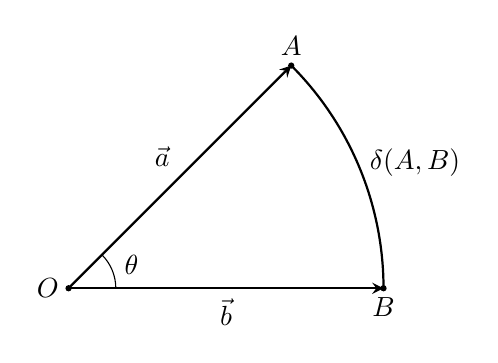
\begin{tikzpicture}[scale=2,>=stealth]
\coordinate (O) at (0,0);
\coordinate (A) at (1.414, 1.414);
\coordinate (B) at (2,0);
\fill (O) circle (0.02) node[left] {$O$};
\fill (A) circle (0.02) node[above] {$A$};
\fill (B) circle (0.02) node[below] {$B$};
\draw[thick] (B) arc (0:45:2);
\node at (2.2, 0.8) {$\delta(A, B)$};

\draw (0.3,0) arc (0:45:0.3);
\node at (0.4,0.15) {$\theta$};

\draw[thick, ->] (O) -- (A) node[midway, above left] {$\vec{a}$};
\draw[thick, ->] (O) -- (B) node[midway, below] {$\vec{b}$};
\end{tikzpicture}
\end{center}
We denote $\angle AOB = \delta(A, B)$.
The following properties then hold:
\begin{align*}
  \vec{a} \cdot \vec{b} &= \cos (\angle AOB) = \cos \delta(A, B) \\
  |\vec{a} \times \vec{b}| &= \sin \delta(A, B)
\end{align*}

Then:
\begin{align*}
  \cos \alpha &= \frac{(\vec{a} \times \vec{b}) \cdot (\vec{a} \times \vec{c})}{|\vec{a} \times \vec{b}| |\vec{a} \times \vec{c}|} \\
               &= - \frac{(\vec{b} \times \vec{a})(\vec{a} \times \vec{c})}{|\vec{a} \times \vec{b}||\vec{a} \times \vec{c}|} \\
               &= \frac{(\vec{b} \cdot \vec{c})|\vec{a}|^2 - (\vec{b} \cdot \vec{a})(\vec{a} \cdot \vec{c})}{|\vec{a} \times \vec{b}||\vec{a} \times \vec{c}|} \\
  (\cos \alpha)|\vec{a} \times \vec{b}||\vec{a} \times \vec{c}| &= (\vec{b} \cdot \vec{c}) - (\vec{b} \cdot \vec{a})(\vec{a} \cdot \vec{c}) \text{ as $|\vec{a}| = 1$} \\
  \cos \alpha \sin \delta(A, B) \sin \delta(A, C) &= \cos \delta(B, C) - \cos \delta(B, A) \cos \delta(A, C)
\end{align*}
This is an analogue of the cosine rule for spherical triangles.

\subsubsection{Vector Definition of Spheres}
A sphere in $\R^3$ with centre $\vec{a}$ and radius $r \in \R$, $r > 0$ is given by:
\[
  \Sigma=\{\vec{x} \in \R^3 : |\vec{x} - \vec{a}| = r > 0,\ r \in \R\}
\]
This also generalises to $\R^{n}$.
A hypersphere with centre $\vec{a} \in \R^{n}$ and radius $r \in \R$ is given by:
\[
  \Sigma =\{\vec{x} \in \R^{n} : |\vec{x} - \vec{a}| = r > 0,\ r \in \R,\ \vec{a} \in \R^{n}\}
\]
\section{Generalised Real Vectors\texorpdfstring{ -- $\R^{n}$}{}}
\label{generalisedReal}
\subsection{Definitions for Real Vectors}
Thinking of vectors component-wise makes it easier to generalise from 3 to $n$ dimensions.

Define $\R^{n}$ as:
\[
  \R^{n} = \{\vec{x} = (x_1, x_2, \ldots, x_n),\ x_i \in \R\}
\]
We write vectors $\vec{x}, \vec{y} \in \R^{n}$ as:
\[
  \vec{x} = (x_1, x_2, \ldots, x_n),\ \vec{y} = (y_1, y_2, \ldots, y_n)
\]
\subsubsection{Addition}
We define addition as:
\[
  \vec{x} + \vec{y} = (x_1 + y_1, x_2 + y_2, \ldots, x_n + y_n)
\]
\subsubsection{Scalar Multiplication}
We define scalar multiplication, for $\lambda \in \R$ as:
\[
  \lambda \vec{x} = (\lambda x_1, \lambda x_2, \ldots, \lambda x_n)
\]
\subsubsection{Inner Product}
We define the inner product between $\vec{x}$ and $\vec{y}$ as:
\[
  \vec{x} \cdot \vec{y} = \sum_{i}^{} x_i y_i = x_1 y_1 + \cdots + x_n y_n
\]
We can also write:
\[
  \vec{x} \cdot \vec{y} = \delta_{i j} x_i y_j
\]
\begin{remark}[Note]
  If we write vectors in $\R^{n}$ as column vectors, if $\vec{x}, \vec{y} \in \R^{n}$, $\vec{x}^{\trans}$ and $\vec{y}^{\trans}$ will be row vectors and their inner product can be represented as:
  \[
    \vec{x} \cdot \vec{y} = \vec{x}^{\trans} \vec{y} =
    \begin{pmatrix}
    x_1 & \cdots & x_n \\
    \end{pmatrix}
    \begin{pmatrix}
    y_1 \\
    \vdots \\
    y_n \\
    \end{pmatrix}
    = \sum_{i}^{} x_i y_i
  \]
\end{remark}
\subsubsection{Canonical Basis}
The \textit{canonical basis} of $\R^{n}$ is $\{\vec{e}_1, \vec{e}_2, \ldots, \vec{e}_n\}$ where:
\[
  \vec{e}_1 = (1, 0, \ldots, 0),\ \vec{e}_2 = (0, 1, \ldots, 0),\ \cdots,\ \vec{e}_n = (0, 0, \ldots, 1)
\]
This is an orthonormal basis so:
\[
  \vec{e}_i \cdot \vec{e}_j = \delta_{i j}
\]
Any $x \in \R^{n}$ can be written as:
\[
  \vec{x} = \sum_{i}^{} x_i \vec{e}_i
\]

Components of $\vec{x} = (x_1, x_2, \ldots, x_n)$ can be determined from:
\[
  x_i = \vec{e}_i \cdot \vec{x}
\]
\subsubsection{Generalised Levi-Civita Epsilon}
Define $\levi_{a_1 a_2 \ldots}$ (with $n$ indices) as an extension to the Levi-Civita epsilon.
\[
  \levi_{a_1 a_2 \ldots a_n} = \begin{cases}
  1 & (a_1, a_2, \ldots, a_n) \text{ is an even permutation of }(1, 2, \ldots, n) \\
  -1 & (a_1, a_2, \ldots, a_n) \text{ is an odd permutation of }(1, 2, \ldots, n) \\
  0 & \text{ otherwise}
  \end{cases}
\]
\subsection{Scalar Cross Product}
\label{scalarCrossProduct}
In $\R^{2}$ we can use this to define an additional scalar product:
\[
  [\vec{a}, \vec{b}] = \levi_{i j}a_i b_j = a_1 b_2 - a_2 b_1
\]
as $\levi_{1 2} = 1$ and $\levi_{2 1} = -1$.

Geometrically this represents the signed area of a parallelogram:
\[
  [\vec{a}, \vec{b}] = |\vec{a}||\vec{b}|\sin\theta
\]
\begin{center}
\begin{tikzpicture}[scale=2,>=stealth]
\coordinate (O) at (0,0);
\coordinate (A) at (2,0);
\coordinate (B) at (1.2,1.2);

\fill[gray!20] (O) -- (A) -- ($(A)+(B)$) -- (B) -- cycle;

\draw (0.3,0) arc (0:45:0.3);
\node at (0.4,0.15) {$\theta$};

\node at (2.3,0.9) {$[\vec{a}, \vec{b}]$};
\draw[->, thick] (O) -- (A) node[midway, below] {$\vec{a}$};
\draw[->, thick] (O) -- (B) node[midway, above left] {$\vec{b}$};

\draw[dashed] (A) -- ($(A)+(B)$);
\draw[dashed] (B) -- ($(A)+(B)$);
\end{tikzpicture}
\end{center}
This is similar to the vector triple product in  $\R^{3}$ which represents the signed volume of a parallelepiped.
\section{Generalised Complex Vectors\texorpdfstring{ -- $\C^{n}$}{}}
\subsection{Definitions for Complex Vectors}
Similarly to in $\R^{n}$ we define $C^{n}$ as:
\[
  \C^{n} = \{\vec{z} = (z_1, z_2, \ldots, z_n): z_i \in \C\}
\]
We write vectors $\vec{z}, \vec{w} \in \C^{n}$ as:
\[
  \vec{z} = (z_1, \ldots, z_n),\ \vec{w} = (w_1, \ldots, w_n)
\]
\subsubsection{Addition}
Exactly as in $\R^{n}$, we define addition as:
\[
  \vec{z} + \vec{w} = (z_1 + w_1, \ldots, z_n + w_n)
\]
\subsubsection{Scalar Multiplication}
We also define scalar multiplication similarly:
\[
  \lambda \vec{z} = (\lambda z_1, \ldots, \lambda z_n)
\]
However, there is important differences depending on if we use real or complex scalars.
\subsubsection{Real Scalars}
If $\lambda \in \R$, $\C^{n}$ is a \textit{real} vector space.
For any $z \in \C^{n}$, $z_j = x_j + iy_j$ so:
\[
  \vec{z} = \sum_{j}^{} x_j \vec{e}_j + \sum_{j}^{} y_j \vec{f}_j
\]
Where:
\[
  \vec{e}_j = \underbrace{(0, 0, \ldots, 1, \ldots, 0)}_{\text{1 in $j$-th position}} \text{ and }
  \vec{f}_j = \underbrace{(0, 0, \ldots, i, \ldots, 0)}_{\text{$i$ in $j$-th position}}
\]
Writing $\vec{z}$ like this is a \textit{real linear combination}.
So the canonical basis for $\C^{n}$ when it is a \textit{real} vector space is:
\[
  \{\vec{e}_1, \vec{e}_2, \ldots, \vec{e}_n, \vec{f}_1, \vec{f}_2, \ldots, \vec{f}_n\}
\]
This means that it has real dimension $2n$.
\subsubsection{Complex Scalars}
If $\lambda \in \C$, $\C^{n}$ is a \textit{complex} vector space.
Since we are allowing complex scalars we can write:
\[
  \vec{f}_j = i \vec{e}_j
\]
and thus:
\[
  \vec{z} = \sum_{j}^{} z_j \vec{e}_j
\]
which is a complex linear combination.
So the canonical basis for $\C^{n}$ as a \textit{complex} vector space is:
\[
  \{\vec{e}_1, \vec{e}_2, \ldots, \vec{e}_n\}
\]
This means that is has dimension $n$ over $\C$.
\subsubsection{Inner Product}
The inner product on $\C^{n}$ is defined by:
\[
  (\vec{z}, \vec{w}) = \sum_{j}^{} z^{*}_{j} w_j
\]
This has the following properties:
\begin{enumerate}
  \item \textbf{Hermitian -} Exchanging $z$ and $w$ takes the conjugate of the output. That is:
    \[
      (w, z) = (z, w)^{*}
    \]
  \item \textbf{Linear/Anti-linear -} It is linear in the second argument and anti-linear in the first argument:
    \begin{align*}
      (\vec{z}, \lambda \vec{w} + \lambda' \vec{w}') &= \lambda(\vec{z}, \vec{w}) + \lambda'(\vec{z}, \vec{w}') \\
      (\mu \vec{z} + \mu' \vec{z}', \vec{w}) &= \mu^{*}(\vec{z}, \vec{w}) + {\mu'}^{*}(\vec{z}', \vec{w})
    \end{align*}
  \item \textbf{Positive Definite}
    \[
      (\vec{z}, \vec{z}) = \sum_{j} |z_j|^2 \geq 0
    \]
    Moreover, $(\vec{z}, \vec{z}) = 0$ if and only if $\vec{z} = \vec{0}$.
\end{enumerate}
\subsubsection{Norm}
We define the norm on $\C^{n}$ as:
\[
  |\vec{z}|^2 = (\vec{z}, \vec{z})
\]
\subsubsection{Orthogonality}
We say that $\vec{z}, \vec{w} \in \C^{n}$  are \textit{orthogonal} if $(\vec{z}, \vec{w}) = 0$.

The standard basis for $\C^{n}$ as a complex vector space is \textit{orthonormal}, that is:
\[
  (\vec{e}_i, \vec{e}_j) = \delta_{i j}\quad\forall 1 \leq i, j \leq n
\]
\subsection{From Complex to Real Inner Products}
For $n = 1$, take $z, w \in \C$, then:
\[
  (z, w) = z^{*}w
\]
Now write $z = a_1 + ia_2, w = b_1 + ib_2$, now associate $z$ and $w$ with the vectors $(a_1, a_2)$ and $(b_1, b_2)$ in $\R^2$.
Then:
\begin{align*}
  z^{*}w &= (a_1 - i a_2)(b_1 + i b_2) \\
         &= (a_1 b_1 + a_2 b_2) + i(a_1 b_2 - a_2 b_1) \\
         &= \vec{a} \cdot \vec{b} + i[\vec{a}, \vec{b}]
\end{align*}
so we can recover both scalar products in $\R^{2}$ from the real and imaginary components.
See \cref{scalarCrossProduct} for a definition of $[\vec{a}, \vec{b}]$.
\section{General Vector Spaces}
\begin{remark}[Recap]\par
Recall the definition and properties of a vector space from \cref{vectorSpaceDef}.

If the scalar multiplication is done by scalars in $\R$ then we have a \textit{real vector space}.
If the scalar multiplication is done by scalars in $\C$ then we have a \textit{complex vector space}.

If we take a real vector space $V$, and consider elements $\vec{v}_1, \ldots, \vec{v}_r \in V$ we can write a \textit{linear combination} of those elements:
\[
  \lambda_1 \vec{v}_1 + \lambda_2 \vec{v}_2 + \cdots + \lambda_r \vec{v}_r \in V \quad \lambda_i \in \R
\]
The \textit{span} of $\{\vec{v}_1, \vec{v}_2, \ldots, \vec{v}_r\}$ is:
\[
  \Span\{\vec{v}_1, \vec{v}_2, \ldots, \vec{v}_r\} = \left\{\sum_{i}^{} \lambda_i \vec{v}_i : \lambda_i \in \R\right\}
\]
\end{remark}
\subsection{Subspaces}
\begin{definition}[Subspace]
  A \textit{subspace} of $V$ is a subset of $V$ that is itself a vector space.

  Equivalently, a non-empty subset $U \subseteq V$ is a subspace if it satisfies that for every pair of vectors $\vec{v}, \vec{w} \in U$ and for any pair of scalars $\lambda, \mu \in \R$ then, $\lambda \vec{v} + \mu \vec{w} \in U$.
\end{definition}
In particular, for any $\vec{v}_1, \ldots, \vec{v}_r$, their span, $\Span\{\vec{v}_1, \ldots, \vec{v}_2\}$, is a subspace of $V$.
The two trivial subspaces of any vector space $V$ are $V$ itself and $\{\vec{0}\}$.

\subsection{Linear Independence and Dependence}
\begin{definition}[Linearly Independant]
  Consider a vector space $V$ and vectors $\vec{v}_1, \ldots, \vec{v}_n \in V$.
  Take a linear combination of these vectors and set it to $\vec{0}$:
  \[
    \lambda_1 \vec{v}_1 + \cdots + \lambda_n \vec{v}_n = \vec{0} \quad \lambda_i \in \R \text{ or } \C
  \]
  If this implies that $\lambda_i = 0$ for all $i$ then the vectors that we are considering are said to be \textit{linearly independent}.
  Otherwise if $\lambda_1 \vec{v}_1 + \cdots + \lambda_n \vec{v}_n = \vec{0}$ with at least one $\lambda_i \neq 0$ then the vectors are \textit{linearly dependant}.
\end{definition}

If a set of vectors are linearly independent then we cannot construct one of the vectors as a linear combination of the others.
\begin{example}
  \begin{enumerate}
    \item $\{\underbrace{(1, 0)}_{\vec{v}_1}, \underbrace{(0, 1)}_{\vec{v}_2}, \underbrace{(0, 2)}_{\vec{v}_3}\} \subseteq \R^2$ is linearly dependant as $\vec{v}_3 = 2\vec{v}_2$ so $0\vec{v}_1 - 2\vec{v}_2 + \vec{v}_3 = \vec{0}$.
    \item $\{\underbrace{(1, 0)}_{\vec{v}_1}, \underbrace{(0, 1)}_{\vec{v}_2}\} \subseteq \R^2$ is linearly independent as $\lambda_1 \vec{v}_1 + \lambda_2 \vec{v}_2 = \vec{0} \implies \lambda_1 = \lambda_2 = 0$
    \item Any set containing $\vec{0}$ is \textit{linearly dependant} as we can set the scalar for $\vec{0}$ to anything non-zero and then all other scalars to 0.
    \item In $\R^3$, $\vec{a}, \vec{b}, \vec{c}$ are linearly independent if and only if $\vec{a} \cdot (\vec{b} \times \vec{c}) \neq 0$.
      This can be seen by considering the volume of the parallelepiped spanned by the three vectors.
 \end{enumerate}
\end{example}
\subsection{Inner Products}
For $\vec{v}, \vec{w} \in V$, denote their inner product by $\vec{v} \cdot \vec{w}$ or $(\vec{v} \cdot \vec{w})$.
This has the following properties:
\begin{enumerate}
  \item $(\vec{v}, \vec{w}) \in \R \text{ or } \C$ depending on if we are in a real or complex vector space.
  \item \textbf{Hermitian -} $(\vec{v}, \vec{w}) = (\vec{w}, \vec{v})^{*}$.
    If it is a real vector space $(\vec{w}, \vec{v})^{*} = (\vec{w}, \vec{v})$ so this reduces to symmetry.
  \item \textbf{Linear/Anti-linear -} It is linear in the second argument and anti-linear in the first argument:
    \begin{align*}
      (\vec{v}, \lambda \vec{w} + \lambda' \vec{w}') &= \lambda(\vec{v}, \vec{w}) + \lambda' (\vec{v}, \vec{w}') \\
      (\mu \vec{v} + \mu \vec{v}', \vec{w}) &= \mu(\vec{v}, \vec{w}) + {\mu'}^{*}(\vec{v}', \vec{w})
    \end{align*}
    If this is a real vector space then this reduces to linearity in both arguments.
  \item \textbf{Positive Definite}
    \[
      (\vec{v}, \vec{v}) \geq 0 \text{ and } ((\vec{v}, \vec{v}) = 0 \iff \vec{v} = \vec{0})
    \]
\end{enumerate}
\begin{proposition}
  If $\vec{v}_1, \vec{v}_2, \ldots, \vec{v}_n$ are non-zero and orthogonal then they are linearly independent.
\end{proposition}
\begin{proof}
  Consider the linear combination:
  \[
    \sum_{i}^{} \alpha_i \vec{v}_i = \vec{0}
  \]
  Then,
  \begin{align*}
    \left(\vec{v}_j, \sum_{i}^{} \alpha_i \vec{v}_i\right) &= \sum_{i}^{} \alpha_i (\vec{v}_j, \vec{v}_i) \text{ (By linearity of second argument)}\\
                                                           &= \alpha_j (\vec{v}_j, \vec{v}_j) \text{ (Because of orthogonality $(\vec{v}_j, \vec{v}_i) = 0$ for $i \neq j$)}\\
                                                           &= \alpha_j |\vec{v}_j|^2
  \end{align*}
  So $\alpha_j|\vec{v}_j|^2 = 0$.
  From positive definiteness we have that $\alpha_j\vec{v}_j = \vec{0}$ but $\vec{v}_j \neq \vec{0}$ so $\alpha_j = 0$.
  This argument holds for all $j$ so $\alpha_j = 0$ for all $j$ so they must be linearly independent by definition.
\end{proof}
\subsection{Bases and Dimension}
\begin{definition}[Basis]
  For a vector space $V$, a \textit{basis} is a set $B = \{\vec{e}_1, \ldots, \vec{e}_n\}$ such that:
  \begin{enumerate}
    \item $B$ \textit{spans} $V$, that is, any $\vec{v} \in V$ can be written as a linear combination of vectors in $B$:
      \[
        \vec{v} = \sum_{i=1}^{n} v_i \vec{e}_i
      \]
    \item $B$ is linearly independent.
      This implies that the coefficients of the linear combination in \textbf{i} are always \textbf{unique}.
      That is, there is only one way to express a particular vector as a linear combination of basis vectors.
      We then call these coefficients, $v_i$, the \textit{components} of $\vec{v}$ with respect to the basis $B$.
  \end{enumerate}
\end{definition}
\begin{theorem}
  If $B_1$ and $B_2$ are both bases for a vector space $V$, then $|B_1| = |B_2|$.
  \label{basesSize}
\end{theorem}
\begin{definition}[Dimension]
  The number of elements in any basis for $V$ is called the \textit{dimension} of $V$.
\end{definition}
\begin{remark}[Note]
  We can use any basis of $V$ to determine its dimension as by \cref{basesSize} the size of all bases for a particular vector space must be equal.
\end{remark}
\begin{proposition}
  Consider a vector space $V$ of dimension $n$,
  \begin{enumerate}
    \item If $Y = \{\vec{w}_1, \ldots, \vec{w}_m\}$ spans $V$ with $m \geq n$ then if $m = n$, $Y$ is a basis for $V$.
      Otherwise, if $m > n$, then we can remove vectors from $Y$ until we have $n$ elements to get a basis for $V$.
    \item If $X = \{\vec{u}_1, \ldots, \vec{u}_k\}$ is linearly independent with $k \leq n$ then if $k = n$, $X$ is a basis for $V$.
      Otherwise, if $k < n$ then it cannot be a basis but we can add more linearly independent vectors until we have $n$ elements to get a basis for $V$.
  \end{enumerate}
\end{proposition}
\begin{remark}
  There will always exists a basis for any vector space, regardless of if it has finite or infinite dimension.
\end{remark}
\end{document}
